% Options for packages loaded elsewhere
\PassOptionsToPackage{unicode}{hyperref}
\PassOptionsToPackage{hyphens}{url}
%
\documentclass[
]{article}
\usepackage{amsmath,amssymb}
\usepackage{iftex}
\ifPDFTeX
  \usepackage[T1]{fontenc}
  \usepackage[utf8]{inputenc}
  \usepackage{textcomp} % provide euro and other symbols
\else % if luatex or xetex
  \usepackage{unicode-math} % this also loads fontspec
  \defaultfontfeatures{Scale=MatchLowercase}
  \defaultfontfeatures[\rmfamily]{Ligatures=TeX,Scale=1}
\fi
\usepackage{lmodern}
\ifPDFTeX\else
  % xetex/luatex font selection
\fi
% Use upquote if available, for straight quotes in verbatim environments
\IfFileExists{upquote.sty}{\usepackage{upquote}}{}
\IfFileExists{microtype.sty}{% use microtype if available
  \usepackage[]{microtype}
  \UseMicrotypeSet[protrusion]{basicmath} % disable protrusion for tt fonts
}{}
\makeatletter
\@ifundefined{KOMAClassName}{% if non-KOMA class
  \IfFileExists{parskip.sty}{%
    \usepackage{parskip}
  }{% else
    \setlength{\parindent}{0pt}
    \setlength{\parskip}{6pt plus 2pt minus 1pt}}
}{% if KOMA class
  \KOMAoptions{parskip=half}}
\makeatother
\usepackage{xcolor}
\usepackage[margin=1in]{geometry}
\usepackage{color}
\usepackage{fancyvrb}
\newcommand{\VerbBar}{|}
\newcommand{\VERB}{\Verb[commandchars=\\\{\}]}
\DefineVerbatimEnvironment{Highlighting}{Verbatim}{commandchars=\\\{\}}
% Add ',fontsize=\small' for more characters per line
\usepackage{framed}
\definecolor{shadecolor}{RGB}{248,248,248}
\newenvironment{Shaded}{\begin{snugshade}}{\end{snugshade}}
\newcommand{\AlertTok}[1]{\textcolor[rgb]{0.94,0.16,0.16}{#1}}
\newcommand{\AnnotationTok}[1]{\textcolor[rgb]{0.56,0.35,0.01}{\textbf{\textit{#1}}}}
\newcommand{\AttributeTok}[1]{\textcolor[rgb]{0.13,0.29,0.53}{#1}}
\newcommand{\BaseNTok}[1]{\textcolor[rgb]{0.00,0.00,0.81}{#1}}
\newcommand{\BuiltInTok}[1]{#1}
\newcommand{\CharTok}[1]{\textcolor[rgb]{0.31,0.60,0.02}{#1}}
\newcommand{\CommentTok}[1]{\textcolor[rgb]{0.56,0.35,0.01}{\textit{#1}}}
\newcommand{\CommentVarTok}[1]{\textcolor[rgb]{0.56,0.35,0.01}{\textbf{\textit{#1}}}}
\newcommand{\ConstantTok}[1]{\textcolor[rgb]{0.56,0.35,0.01}{#1}}
\newcommand{\ControlFlowTok}[1]{\textcolor[rgb]{0.13,0.29,0.53}{\textbf{#1}}}
\newcommand{\DataTypeTok}[1]{\textcolor[rgb]{0.13,0.29,0.53}{#1}}
\newcommand{\DecValTok}[1]{\textcolor[rgb]{0.00,0.00,0.81}{#1}}
\newcommand{\DocumentationTok}[1]{\textcolor[rgb]{0.56,0.35,0.01}{\textbf{\textit{#1}}}}
\newcommand{\ErrorTok}[1]{\textcolor[rgb]{0.64,0.00,0.00}{\textbf{#1}}}
\newcommand{\ExtensionTok}[1]{#1}
\newcommand{\FloatTok}[1]{\textcolor[rgb]{0.00,0.00,0.81}{#1}}
\newcommand{\FunctionTok}[1]{\textcolor[rgb]{0.13,0.29,0.53}{\textbf{#1}}}
\newcommand{\ImportTok}[1]{#1}
\newcommand{\InformationTok}[1]{\textcolor[rgb]{0.56,0.35,0.01}{\textbf{\textit{#1}}}}
\newcommand{\KeywordTok}[1]{\textcolor[rgb]{0.13,0.29,0.53}{\textbf{#1}}}
\newcommand{\NormalTok}[1]{#1}
\newcommand{\OperatorTok}[1]{\textcolor[rgb]{0.81,0.36,0.00}{\textbf{#1}}}
\newcommand{\OtherTok}[1]{\textcolor[rgb]{0.56,0.35,0.01}{#1}}
\newcommand{\PreprocessorTok}[1]{\textcolor[rgb]{0.56,0.35,0.01}{\textit{#1}}}
\newcommand{\RegionMarkerTok}[1]{#1}
\newcommand{\SpecialCharTok}[1]{\textcolor[rgb]{0.81,0.36,0.00}{\textbf{#1}}}
\newcommand{\SpecialStringTok}[1]{\textcolor[rgb]{0.31,0.60,0.02}{#1}}
\newcommand{\StringTok}[1]{\textcolor[rgb]{0.31,0.60,0.02}{#1}}
\newcommand{\VariableTok}[1]{\textcolor[rgb]{0.00,0.00,0.00}{#1}}
\newcommand{\VerbatimStringTok}[1]{\textcolor[rgb]{0.31,0.60,0.02}{#1}}
\newcommand{\WarningTok}[1]{\textcolor[rgb]{0.56,0.35,0.01}{\textbf{\textit{#1}}}}
\usepackage{longtable,booktabs,array}
\usepackage{calc} % for calculating minipage widths
% Correct order of tables after \paragraph or \subparagraph
\usepackage{etoolbox}
\makeatletter
\patchcmd\longtable{\par}{\if@noskipsec\mbox{}\fi\par}{}{}
\makeatother
% Allow footnotes in longtable head/foot
\IfFileExists{footnotehyper.sty}{\usepackage{footnotehyper}}{\usepackage{footnote}}
\makesavenoteenv{longtable}
\usepackage{graphicx}
\makeatletter
\def\maxwidth{\ifdim\Gin@nat@width>\linewidth\linewidth\else\Gin@nat@width\fi}
\def\maxheight{\ifdim\Gin@nat@height>\textheight\textheight\else\Gin@nat@height\fi}
\makeatother
% Scale images if necessary, so that they will not overflow the page
% margins by default, and it is still possible to overwrite the defaults
% using explicit options in \includegraphics[width, height, ...]{}
\setkeys{Gin}{width=\maxwidth,height=\maxheight,keepaspectratio}
% Set default figure placement to htbp
\makeatletter
\def\fps@figure{htbp}
\makeatother
\setlength{\emergencystretch}{3em} % prevent overfull lines
\providecommand{\tightlist}{%
  \setlength{\itemsep}{0pt}\setlength{\parskip}{0pt}}
\setcounter{secnumdepth}{-\maxdimen} % remove section numbering
\ifLuaTeX
  \usepackage{selnolig}  % disable illegal ligatures
\fi
\IfFileExists{bookmark.sty}{\usepackage{bookmark}}{\usepackage{hyperref}}
\IfFileExists{xurl.sty}{\usepackage{xurl}}{} % add URL line breaks if available
\urlstyle{same}
\hypersetup{
  pdftitle={Teknisk beskrivelse og dokumentation},
  hidelinks,
  pdfcreator={LaTeX via pandoc}}

\title{Teknisk beskrivelse og dokumentation}
\author{}
\date{\vspace{-2.5em}2024-02-26}

\begin{document}
\maketitle

\hypertarget{data}{%
\subsection{Data}\label{data}}

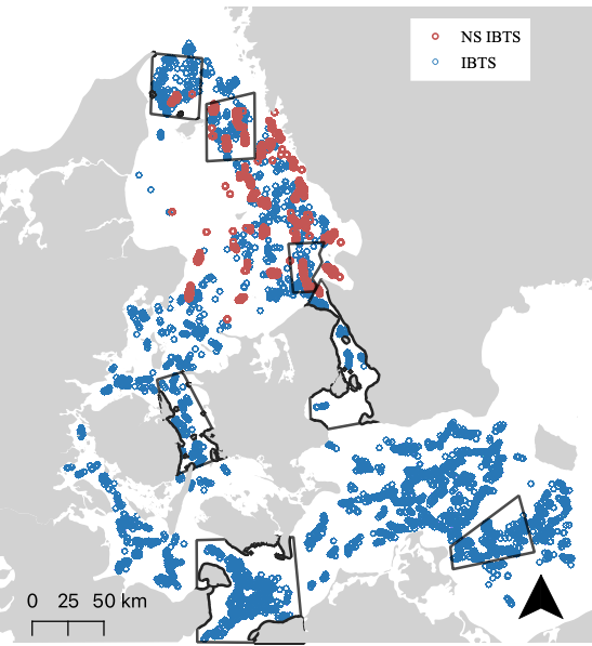
\includegraphics[width=0.3\linewidth,style="float:right; padding:10px"]{omraader}
Data er hentet fra ICES' Database of Trawl Surveys
(\href{https://www.ices.dk/data/data-portals/Pages/DATRAS.aspx}{DATRAS}).
For at dække hele Danmark, er to surveys brugt:

\begin{itemize}
\tightlist
\item
  North Sea International Bottom Trawl Survey (NS-IBTS)
\item
  Baltic International Trawl Survey (BITS).
\end{itemize}

7 polygoner/områder er lavet i QGIS og data er klippet til hvert område.
Dvs. der nu er 7 datasæt: et over hvert område. Hvert område er valgt ud
fra følgende:

\begin{itemize}
\tightlist
\item
  Der skal være nok hauls, der går langt nok tilbage i tiden
\item
  Mange datapunkter (hauls)
\item
  Repræsentere, så vidt muligt, forskellige fysiske parametre
\end{itemize}

En shape-fil af havbundssediment
(\href{https://metadata.helcom.fi/geonetwork/srv/eng/catalog.search\#/metadata/ab71bbf8-eacc-4a93-9504-46210da8fe6d}{DHI,
EuSeaMap, BALANCE}) tilføjes og klippes til, så det passer til
områderne, for på den måde senere at kunne tilføje en kolonne i
attributtabellen om sedimenttype. Billedet til højre viser placeringen
af områder samt hauls fra hhv. NS-IBTS og BITS.

\hypertarget{data-rensning-og-pruxe6perering}{%
\subsection{Data rensning og
præperering}\label{data-rensning-og-pruxe6perering}}

\textbf{(mange af de valg der er taget, i forhold til rensning af data
er taget på baggrund af en masse deskriptiv statistik). Data rensning er
dokumenteret i et R-script.}

Derudover inddeles hver art i tre størrelser ud fra både biologiske
kriterier samt min/maks længder for fangst (se skema i app) For hvert
område/art/størrelse er følgende datapræparering/rensning foretaget:

\begin{itemize}
\tightlist
\item
  Kun kvartal 1 og 4
\item
  Kun \textgreater{} år 2000
\item
  Der laves en ny kolonne med et ''unikt'' haul ID, da der ellers tælles
  fra 1 ved hvert nyt år.
\item
  Alle længdeklasser skal repræsenteres, så der tilføjes ''0'' i de
  klasser, der ikke er fanget i haulet.
\item
  En ny kolonne tilføjes med den summerede ''CPUE\_number\_per\_hour''
  for hvert unikt haul af den specifikke kombination af art,
  størrelsesklasse og område.
\item
  Et nyt datasæt (.csv) gemmes for hver art og en kolonne (source) der
  fortæller hvilket område og størrelse der er tale om. F.eks.
  øresund\_codJ (for juvenile torsk i øresund). I alt \textbf{6
  csv-filer}.
\end{itemize}

Tabellen nedenfor viser antallet af hauls i hvert område efter
datarensning.

\begin{longtable}[]{@{}lc@{}}
\toprule\noalign{}
Område & Antal hauls \\
\midrule\noalign{}
\endhead
\bottomrule\noalign{}
\endlastfoot
Nordlige Kattegat & 154 \\
Kattegat, vest for Læsø & 225 \\
Kattegat, nord for Øresund & 77 \\
Øresund & 143 \\
Storebælt & 231 \\
Mecklenburg Bugten & 372 \\
Østersøen, sydvest for Bornholm & 260 \\
\end{longtable}

\hypertarget{generalised-additive-mixed-models-gamm}{%
\subsection{Generalised Additive Mixed Models
(GAMM)}\label{generalised-additive-mixed-models-gamm}}

De nye csv-filer bruges til at lave GAMM-modellerne. Nedstående er et
eksempel på en model i R for juvenile rødspætter i Øresund:

\begin{Shaded}
\begin{Highlighting}[]
\NormalTok{mod.plaiceJ }\OtherTok{\textless{}{-}} \FunctionTok{gam}\NormalTok{(cpue }\SpecialCharTok{\textasciitilde{}}
\NormalTok{                     period }\SpecialCharTok{+}
                     \FunctionTok{s}\NormalTok{(depth, }\AttributeTok{k =} \DecValTok{15}\NormalTok{) }\SpecialCharTok{+} 
                     \FunctionTok{s}\NormalTok{(Gear, }\AttributeTok{bs=} \StringTok{"re"}\NormalTok{) }\SpecialCharTok{+} 
\NormalTok{                     Quarter }\SpecialCharTok{+} 
\NormalTok{                     SedimentDK, }
                   \AttributeTok{data=} \FunctionTok{subset}\NormalTok{(dat\_plaice, loc}\SpecialCharTok{==} \StringTok{"øresund\_plaiceJ"}\NormalTok{), }\AttributeTok{family =}\NormalTok{ tw)}

\NormalTok{mod.plaiceJ }\OtherTok{\textless{}{-}} \FunctionTok{get.mini.model}\NormalTok{(mod. plaiceJ, }\AttributeTok{check.terms =} \FunctionTok{c}\NormalTok{(}\StringTok{"period"}\NormalTok{, }\StringTok{"depth"}\NormalTok{, }\StringTok{"Quarter"}\NormalTok{, }\StringTok{"SedimetnDK"}\NormalTok{))}
\end{Highlighting}
\end{Shaded}

Hvor

\begin{itemize}
\tightlist
\item
  \texttt{cpue} er responsvariablen og er den summerede
  CPUE\_number\_per\_hour for alle længder af arten i størrelsesgruppen
  i et haul.
\item
  \texttt{period} er en af følgende perioder: 2000-2005, 2006-2012,
  2013-2018, 2019-2024 (OBS der er kun data inkluderet til og med 2022)
\item
  \texttt{s(depth)} er dybden der er blevet trawlet på
\item
  \texttt{s(Gear)} er typen af gear der er brugt (læs mere på ICES
  hjemmeside)
\item
  \texttt{Quarter} er kvartalet, dvs enten kvartal 1 eller 4
\item
  \texttt{SedimentDK} er sedimenttypen. Der er fem forskellige typer.
  Sedimenttypen er identificeret på baggrund af ovennævnte sedimentkort
  samt longitude og latitude for de enkelte hauls.
\end{itemize}

\texttt{get.mini.model} henviser til scriptet \textbf{funcs.R}, som
finder den bedste, mindst komplekse model. Med modellerne udregnes nu en
\emph{''predicted CPUE''} og en \emph{''predicted standard deviation''}.
De gemmes som \textbf{newdat.rds}, så model-resultaterne kan bruges i
shiny appen. I alt er lavet 126 modeller. Nogle modeller har ikke kunne
konvergere og kan ses i tabellen nedenunder. Alle scripts kan findes på
\href{https://github.com/lbering/Shiny-app}{github}.

\hypertarget{modeller-med-warnings}{%
\paragraph{Modeller med warnings}\label{modeller-med-warnings}}

\begin{longtable}[]{@{}
  >{\raggedright\arraybackslash}p{(\columnwidth - 2\tabcolsep) * \real{0.4583}}
  >{\raggedright\arraybackslash}p{(\columnwidth - 2\tabcolsep) * \real{0.3333}}@{}}
\toprule\noalign{}
\endhead
\bottomrule\noalign{}
\endlastfoot
\textbf{Område} & \textbf{Art og størrelse} \\
Nordlige Kattegat & \begin{minipage}[t]{\linewidth}\raggedright
\begin{itemize}
\tightlist
\item
  Voksne brisling
\end{itemize}
\end{minipage} \\
Kattegat, vest for Læsø & \begin{minipage}[t]{\linewidth}\raggedright
\begin{itemize}
\tightlist
\item
  Juvenile skrubber
\end{itemize}
\end{minipage} \\
Kattegat, nord for Øresund & \begin{minipage}[t]{\linewidth}\raggedright
\begin{itemize}
\tightlist
\item
  Voksne hvilling
\item
  Unge skrubber
\item
  Juvenile skrubber
\end{itemize}
\end{minipage} \\
Øresund & \begin{minipage}[t]{\linewidth}\raggedright
\begin{itemize}
\tightlist
\item
  Juvenile skrubber
\item
  Juvenile rødspætter
\end{itemize}
\end{minipage} \\
Storebælt & \begin{minipage}[t]{\linewidth}\raggedright
\begin{itemize}
\tightlist
\item
  Voksne torsk
\item
  Voksne brisling
\item
  Voksne hvilling
\item
  Juvenile skrubber
\end{itemize}
\end{minipage} \\
Mecklenburg Bugten & \begin{minipage}[t]{\linewidth}\raggedright
\begin{itemize}
\tightlist
\item
  Juvenile rødspætter
\item
  Juvenile brisling
\item
  Juvenile skrubber
\item
  Voksne brisling
\item
  Voksne hvilling
\end{itemize}
\end{minipage} \\
Østersøen, sydvest for Bornholm &
\begin{minipage}[t]{\linewidth}\raggedright
\begin{itemize}
\tightlist
\item
  Voksne torsk
\item
  Voksne brisling
\item
  Voksne hvilling
\end{itemize}
\end{minipage} \\
\end{longtable}

\end{document}
